\section{The Slack Principle}\label{sec:slack}

\Cref{lem:bidding} and \cref{prop:master} price the chokepoint. On our reading of the record since 2019 (\cref{sec:evidence}), Europe's premium has been negative, and Washington has still asked Europe for a great deal. A patron can obtain the holder's surplus over exit, plus whatever it can threaten that does not depend on the holder's alignment. We state this for any rule that settles Europe's price at the end of a period, so that one result covers the bidding benchmark, bargaining under rupture risk, hold-up and price driving.

\subsection{Bite, budgets and assurance}\label{sec:slackprinciple}

Consider one period in which Europe is aligned and its premium is $Q$. Washington has finitely many demands. Demand $k$ costs Europe $t_k>0$ and is worth $w_k>0$ to the United States. A concession is \emph{reversible} if exit would undo it, so that it lowers Europe's aligned payoff and leaves its exit payoff unchanged. A concession is \emph{sunk} if it lowers both payoffs: payments, purchases, and transfers of assets or of control over them. \Cref{sec:linkage} shows that which concessions are reversible is itself a choice of Washington's.

\paragraph{Settlement.} At the end of the period Europe's price is settled at the premium then prevailing. Let $\mathcal P(q)$ be Europe's payoff from the settlement, relative to the aligned status quo, when its premium is $q$, and let $-\mathcal P(q)$ be Washington's. We require three properties: (S1) $\mathcal P(q)\ge q$, since Europe can always exit; (S2) $\mathcal P$ is nondecreasing; and (S3) $\mathcal P(q')-\mathcal P(q)\le q'-q$ for $q\le q'$, so that a higher premium never raises Europe's price by more than itself. Four settlements in this paper satisfy them while Washington retains Europe: the bidding payment $\mathcal P(q)=\pos{q}$ (\cref{lem:bidding}); bargaining under rupture risk, $\mathcal P(q)=\max\{q,\psi(q+\beta(V-q))\}$ (\cref{prop:master}), a maximum of affine functions with slopes $1$ and $\psi(1-\beta)$; hold-up with constant disagreement costs, which adds $(1-\psi)N$ to the second term (\cref{prop:pain}); and price driving, $\mathcal P(q)=\pos{q+\bar b_C-Q}$ (\cref{rem:spite}). Europe's \emph{surplus over exit} is $\Lambda_{\mathcal P}=\mathcal P(Q)-Q\ge 0$. In the bidding benchmark it is the slack $\Lambda=\pos{-Q}$.

\paragraph{Instruments.} Washington backs its demands with instruments (\cref{sec:security}). Withdrawing a set $J$ of instruments from an aligned Europe for the period lowers Europe's aligned payoff by $\Delta^A(J)$ and its exit payoff by $\Delta^X(J)$, with $0\le\Delta^X(J)\le\Delta^A(J)$ and both nondecreasing in $J$. We call
\[
u(J)=\Delta^X(J)\qquad\text{and}\qquad d(J)=\Delta^A(J)-\Delta^X(J)
\]
the unconditional and conditional parts of $J$. The conditional part is what Europe would lose by exiting anyway (for a single instrument, the $d_j$ of \cref{eq:Q}). The unconditional part is what Washington would still provide to an exited Europe and can threaten to take away. We impose no additivity: the AI instrument and US force posture may be complements or substitutes in Europe's payoff.

\paragraph{Ultimatums.} Washington's credible set $J^c$ is fixed at the start of the period, and no instrument outside it can be withdrawn. Washington issues \emph{adaptive ultimatums}: any sequence of demands, each naming unconceded demands and a threat set of instruments not yet withdrawn, each chosen after seeing Europe's earlier responses. If Europe refuses, Washington executes the threat at direct cost $e(J)\ge 0$, and executed instruments stay withdrawn for the period, so a threat once carried out is \emph{spent}. A threat that deters is not spent and can back the next demand. If $J_w$ has been withdrawn and Europe has made reversible concessions $T_{\mathrm r}$ and sunk ones $T_{\mathrm s}$, the settlement is played at the premium $Q+d(J_w)+T_{\mathrm r}$, and Europe receives $-\Delta^A(J_w)-T_{\mathrm r}-T_{\mathrm s}+\mathcal P(Q+d(J_w)+T_{\mathrm r})$. For a set $S$ of concessions, $T_{\mathrm r}(S)$ and $T_{\mathrm s}(S)$ are its reversible and sunk totals and $W(S)=\sum_{k\in S}w_k$ its value to Washington. Executing $J$ costs Washington $e(J)$ plus the rise in the settlement, which by (S3) is at most $d(J)$. After any history, executing a further set raises the premium by at most $\Delta^A(J^c)$, since $0\le d\le\Delta^A$. So if $e$ is nondecreasing, every subset of $J^c$ stays credible after every history when $\bar m_U\ge e(J^c)+\Delta^A(J^c)$, a condition the attainment claims below use and the bounds do not.

\begin{proposition}[Slack principle]\label{prop:slack}
Let the settlement $\mathcal P$ satisfy (S1)--(S3), let $\Lambda_{\mathcal P}=\mathcal P(Q)-Q$, and let
\[
B(J)=\Delta^A(J)-\big[\mathcal P\big(Q+d(J)\big)-\mathcal P(Q)\big],\qquad \varrho(T)=T-\big[\mathcal P(Q+T)-\mathcal P(Q)\big].
\]
No instrument outside $J^c$ can be withdrawn during the period, executing a withdrawal of $J$ costs the United States $e(J)\ge 0$ directly, and the United States retains Europe after every history.
\begin{enumerate}[label=(\alph*)]
\item \emph{Bite.} Refusing an ultimatum backed by $J$, issued when nothing has been conceded or withdrawn, costs Europe $B(J)$, net of the change in its settlement. $B$ is nondecreasing in $J$, and
\[ B(J)\le u(J)+\min\{d(J),\Lambda_{\mathcal P}\}, \]
with equality if the withdrawal holds Europe to its outside option ($\mathcal P(Q+d(J))=Q+d(J)$) or leaves its settlement unchanged ($\mathcal P(Q+d(J))=\mathcal P(Q)$). In the bidding benchmark equality always holds, $B(J)=u(J)+\min\{d(J),\Lambda\}$, and if $Q\ge 0$ only unconditional parts bite.
\item \emph{Reversible concessions.} Europe's net loss from reversible concessions totalling $T$ is $\varrho(T)\le\min\{T,\Lambda_{\mathcal P}\}$, with equality in the bidding benchmark. Faced with a single ultimatum that asks for reversible concessions $T_{\mathrm r}$ and sunk concessions $T_{\mathrm s}$ and is backed by $J$, Europe accepts if and only if $\varrho(T_{\mathrm r})+T_{\mathrm s}\le B(J)$.
\item \emph{One budget.}
  \begin{enumerate}[label=(\roman*)]
  \item In every subgame-perfect equilibrium of every adaptive sequence of ultimatums, Europe's total net loss is at most $B(J^c)$. Conditional instruments share one budget: $B(J)-u(J)\le\Lambda_{\mathcal P}$ for every $J$, and reversible concessions cost Europe at most $\Lambda_{\mathcal P}$ in total, however they are backed.
  \item The United States' equilibrium payoff is at most
  $V_1=\max\{W(S)-\mathcal P(Q+T_{\mathrm r}(S)):\ \varrho(T_{\mathrm r}(S))+T_{\mathrm s}(S)\le B(J^c)\}$, the payoff of the best single ultimatum backed by $J^c$.
  \item If every subset of $J^c$ stays credible and the United States can commit to a single ultimatum, one bundled ultimatum backed by $J^c$ yields $V_1$. Europe's loss then equals $B(J^c)$ if the United States has a divisible sunk demand of positive value and of size at least $B(J^c)$.
  \end{enumerate}
\item \emph{Assurance.} Without that commitment the United States still obtains $V_1$ if all demands are reversible and $B(J^c)\ge\Lambda_{\mathcal P}$, or if some best single ultimatum contains all of its demands. (In every equilibrium if $e(J)>0$ for every nonempty $J$, as with additive execution costs that are positive for each instrument; in some equilibrium otherwise.) In general it can obtain strictly less. Threats that deter are not spent, so the United States reuses them after Europe concedes, and Europe anticipates this. With one instrument with $d=0$ and $n$ identical sunk demands of cost $\tau$, the United States obtains exactly $n \bmod (b+1)$ of them, where $b=\lfloor B(J^c)/\tau\rfloor$.
\end{enumerate}
\end{proposition}

\Cref{app:proofs} has the proof and \cref{app:numerics} the brute-force checks. The proof uses only (S1)--(S3). Withdrawing a conditional part from an aligned Europe takes away something Europe would lose by exiting anyway, so it raises Europe's premium by $d(J)$. In the bidding benchmark the withdrawal hurts Europe up to $\Lambda$. Beyond $\Lambda$ the premium turns positive and Washington must pay rent to keep Europe aligned, which hands the excess back. A reversible concession works the same way, which is part (b): it lowers only the aligned payoff, so past $\Lambda$ Europe would exit unless compensated. Sunk concessions and unconditional parts escape the cap because they hurt Europe whatever it does.

The same holds whatever settles the price. Under rupture risk, agenda power can lift Europe's price above $\pos{Q}$, and the budget becomes $\Lambda_{\mathcal P}=P^*(Q)-Q$, which grows with $V$ while agenda power binds. It can also be smaller than $\Lambda$: when rupture risk makes Europe concede in the bargaining ($P^*(Q)<0$), threats can extract only the rest of its surplus over exit. Take $Q=-1$, $V=4$, $\beta=0.5$, $\lambda=1$, $r=0.25$ and $\phi=0$. Then $\Lambda=1$ and $\Lambda_{\mathcal P}=2.2$, and withdrawing a conditional part of $3$ costs Europe $1.8$. Whatever agenda power, hold-up or a rival's price driving wins Europe above its outside option, credible conditional threats can claw back, down to the exit premium. The agenda channel of \cref{cor:master}(e) therefore survives only to the extent that Washington lacks credible conditional threats large enough to push Europe to its outside option. Where the second term of $P^*$ binds, the settlement also rises at rate $\psi(1-\beta)$ with the premium, so a reversible concession of $T$ inside the budget costs Europe only $(1-\psi(1-\beta))T$: rupture risk returns part of every reversible concession.

\begin{figure}[t]
\centering
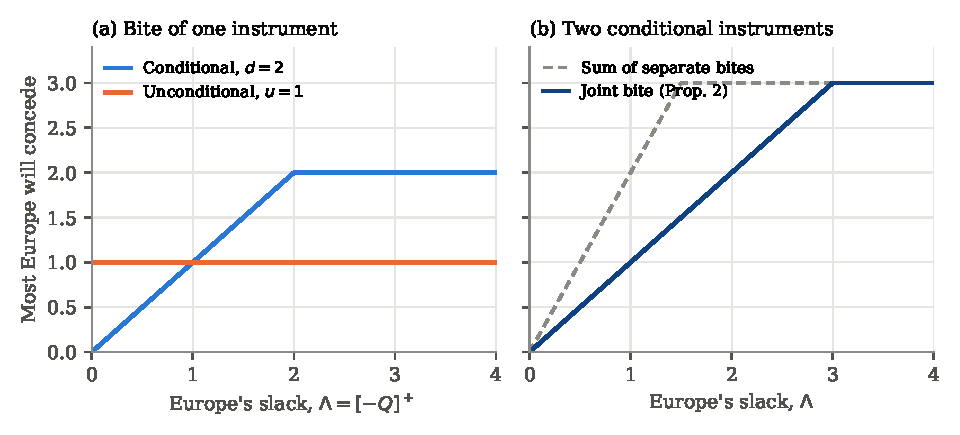
\includegraphics[width=0.95\textwidth]{figures/fig_slack.pdf}
\caption{The slack budget in the bidding benchmark. Panel (a): the bite of a conditional instrument with $d=2$ rises one for one with Europe's slack $\Lambda$ until $\Lambda=2$; an unconditional instrument with $u=1$ bites the same at every $\Lambda$. Panel (b): two conditional instruments with $d=1.5$ each. The sum of their separate bites (dashed) overstates their joint bite $\min\{3,\Lambda\}$ at every $\Lambda<3$. Bites from \cref{prop:slack}(a).}
\label{fig:slack}
\end{figure}

In panel (a) of \cref{fig:slack} the unconditional threat is the smaller one, yet it is the only one that still works as $\Lambda$ falls toward zero. Panel (b) illustrates part (c)(i). A coercer that prices each conditional threat on its own counts the same slack twice: at $\Lambda=1$ the separate bites sum to $2$ and the joint bite is $1$. The bound in (c)(i) needs only a fixed credible set (\cref{app:numerics}). Attaining it needs that set to stay credible after every history, which the cap condition stated before the proposition ensures.

Part (d) is the assurance problem of a coercer that cannot commit to stop demanding. Europe concedes only if everything the unspent threat will extract later stays within the bite. With $b+1$ identical sunk demands, a single ultimatum obtains $b$ of them. The adaptive sequence obtains none. A threat meant to induce compliance works only if the target believes compliance will end it \citep{schelling1966arms}, and \citet{pauly2024damned} shows that the steps that make a threat credible weaken that belief. A staked promise to make no further demand in the period buys the commitment. Stakes cost nothing. Part (d) therefore describes a patron whose cap $\bar m_U$ is small relative to the value of its later demands. Such a patron can gain by issuing an ultimatum it expects Europe to refuse, which burns an instrument that would otherwise back later demands (\cref{app:numerics}).

\begin{corollary}[Rationing]\label{cor:rationing}
In the bidding benchmark, suppose all demands are reversible and either the United States can commit to a single ultimatum or $B(J^c)\ge\Lambda$. Then its optimal demand set solves
\[ \max_{y_k\in\{0,1\}}\ \sum_k w_k y_k-\pos{\textstyle\sum_k t_k y_k-\Lambda}
   \quad\text{s.t.}\quad \min\Big\{\sum_k t_k y_k,\Lambda\Big\}\le B(J^c), \]
with one $y_k$ for each demand $k$. This is the knapsack $\max\sum_k w_k y_k$ s.t.\ $\sum_k t_k y_k\le\min\{\Lambda,B(J^c)\}$ if $B(J^c)<\Lambda$, or if demands are divisible ($y_k\in[0,1]$) and $w_k\le t_k$ for every $k$. In general the United States may exceed $\Lambda$ and pay the excess back as rent. The free capacity $\min\{\Lambda,B(J^c)\}$ falls as $Q$ rises toward $0$. Demands from every issue area draw on it.
\end{corollary}

With a general settlement the objective is $\sum_k w_ky_k-[\mathcal P(Q+\sum_kt_ky_k)-\mathcal P(Q)]$, and capacity is free only where $\mathcal P$ is flat.

